% The kernel-calibrated halo model of intrinsic alignments (HMk): how it is
% built, how well it fits FLAMINGO, and how much it biases Roman.
% Build with assets/build_note.sh of the summary-notes skill.
\documentclass[11pt]{article}

\usepackage[margin=1in]{geometry}
\usepackage{amsmath}
\usepackage{amssymb}
\usepackage{graphicx}
\usepackage{booktabs}
\usepackage{xcolor}
\usepackage{float}
\usepackage[font=small,labelfont=bf,labelsep=period]{caption}
\usepackage[hidelinks]{hyperref}
\setlength{\emergencystretch}{3em}
\renewcommand{\topfraction}{0.9}
\renewcommand{\textfraction}{0.07}
\renewcommand{\floatpagefraction}{0.8}

% Symbols, one macro per object.
\newcommand{\hMpc}{\,h\,{\rm Mpc}^{-1}}
\newcommand{\Msun}{\,h^{-1}M_\odot}
\newcommand{\Plin}{P_{\rm lin}}
\newcommand{\PNL}{P_{\rm NL}}
\newcommand{\bNL}{\beta_{\rm NL}}
\newcommand{\bK}{b_K}
\newcommand{\kmax}{k_{\max}}
\newcommand{\Nc}{\langle N_c\rangle}
\newcommand{\Ns}{\langle N_s\rangle}
\newcommand{\kc}{\kappa_c}
\newcommand{\ks}{\kappa_s}
\newcommand{\Aeff}{A_{\rm eff}}

% =====================================================================
% Numbers
% =====================================================================
% Part 1: results, all in numbers.tex, written by make_numbers.py from
% analysis/halo_kernel/model/hk_model.json, the plots/*/data.json files and
% analysis/cut_validation/fisher_minimize.json. Every macro there carries
% its source in a comment. Set \numbersfinalfalse to print them in red.
%
% Statements of the text that rest on Part 1 (re-check after a refresh):
%   - halo shapes respond to nonlinear gravity about as strongly as matter
%     and much more than halo densities (sections "Summary", "The gravity layer");
%   - the mean-HOD weighting and the split of the halo shape each remove a
%     10 to 20 percent error of the galaxy layer (section "Three corrections");
%   - kappa_r/kappa_d rises with z (section "Three corrections");
%   - HMk with the saturating kernel gradient has the highest goodness-of-fit
%     cuts (sections "Summary", "Goodness of fit");
%   - A is stable in k_max at every z and rises with z (section "Physical checks");
%   - HMk at all z stays below 0.3 in cosmic shear to K0 = 0.6, like TATT;
%     the residual term costs a little at z <= 1.5; the control crosses
%     0.3 in 3x2pt at 0.3 (sections "Summary", "Figure of bias for Roman").
\newif\ifnumbersfinal
\numbersfinaltrue
\newcommand{\refresh}[1]{\ifnumbersfinal#1\else\textcolor{red}{#1}\fi}
% Written by make_numbers.py; do not edit by hand.
\newcommand{\gofWA}{3.27}  % plots/gof/data.json w: sum chi2 / sum nu at k_max 0.52
\newcommand{\gofWC}{11.68}  % plots/gof/data.json w: sum chi2 / sum nu at k_max 0.94
\newcommand{\cutWLo}{0.09}  % plots/gof/data.json w: min GOF cut over the core z
\newcommand{\cutWHi}{0.52}  % plots/gof/data.json w: max GOF cut
\newcommand{\cutWMed}{0.39}  % plots/gof/data.json w: median GOF cut
\newcommand{\gofWgA}{1.41}  % plots/gof/data.json wg: sum chi2 / sum nu at k_max 0.52
\newcommand{\gofWgC}{2.01}  % plots/gof/data.json wg: sum chi2 / sum nu at k_max 0.94
\newcommand{\cutWgLo}{0.16}  % plots/gof/data.json wg: min GOF cut over the core z
\newcommand{\cutWgHi}{2.27}  % plots/gof/data.json wg: max GOF cut
\newcommand{\cutWgMed}{0.52}  % plots/gof/data.json wg: median GOF cut
\newcommand{\gofVoneA}{1.56}  % plots/gof/data.json v1: sum chi2 / sum nu at k_max 0.52
\newcommand{\gofVoneC}{2.77}  % plots/gof/data.json v1: sum chi2 / sum nu at k_max 0.94
\newcommand{\cutVoneLo}{0.22}  % plots/gof/data.json v1: min GOF cut over the core z
\newcommand{\cutVoneHi}{0.94}  % plots/gof/data.json v1: max GOF cut
\newcommand{\cutVoneMed}{0.52}  % plots/gof/data.json v1: median GOF cut
\newcommand{\gofTattA}{5.68}  % plots/gof/data.json tatt: sum chi2 / sum nu at k_max 0.52
\newcommand{\gofTattC}{19.39}  % plots/gof/data.json tatt: sum chi2 / sum nu at k_max 0.94
\newcommand{\cutTattLo}{0.29}  % plots/gof/data.json tatt: min GOF cut over the core z
\newcommand{\cutTattHi}{0.70}  % plots/gof/data.json tatt: max GOF cut
\newcommand{\cutTattMed}{0.29}  % plots/gof/data.json tatt: median GOF cut
\newcommand{\gofLinA}{177.09}  % plots/gof/data.json lin: sum chi2 / sum nu at k_max 0.52
\newcommand{\gofLinC}{810.84}  % plots/gof/data.json lin: sum chi2 / sum nu at k_max 0.94
\newcommand{\cutLinLo}{0.12}  % plots/gof/data.json lin: min GOF cut over the core z
\newcommand{\cutLinHi}{0.12}  % plots/gof/data.json lin: max GOF cut
\newcommand{\cutLinMed}{0.12}  % plots/gof/data.json lin: median GOF cut
\newcommand{\gofEmuA}{33.27}  % plots/gof/data.json emu: sum chi2 / sum nu at k_max 0.52
\newcommand{\gofEmuC}{227.93}  % plots/gof/data.json emu: sum chi2 / sum nu at k_max 0.94
\newcommand{\cutEmuLo}{0.09}  % plots/gof/data.json emu: min GOF cut over the core z
\newcommand{\cutEmuHi}{0.16}  % plots/gof/data.json emu: max GOF cut
\newcommand{\cutEmuMed}{0.11}  % plots/gof/data.json emu: median GOF cut
\newcommand{\gofTabA}{8.52}  % plots/gof/data.json tab: sum chi2 / sum nu at k_max 0.52
\newcommand{\gofTabC}{20.53}  % plots/gof/data.json tab: sum chi2 / sum nu at k_max 0.94
\newcommand{\cutTabLo}{0.22}  % plots/gof/data.json tab: min GOF cut over the core z
\newcommand{\cutTabHi}{0.29}  % plots/gof/data.json tab: max GOF cut
\newcommand{\cutTabMed}{0.25}  % plots/gof/data.json tab: median GOF cut
\newcommand{\respShape}{2.5}  % plots/shape_response/data.json z = 1, shape at k = 0.94
\newcommand{\respDens}{1.6}  % plots/shape_response/data.json z = 1, density at k = 0.94
\newcommand{\respMatter}{3.0}  % plots/shape_response/data.json z = 1, matter at k = 0.94
\newcommand{\respEmu}{1.8}  % plots/shape_response/data.json z = 1, emulator at k = 0.94
\newcommand{\ggBinnedMiss}{16}  % plots/weighting/data.json z = 1: 1 - binned P_GG/P_gg, mean over k = 0.02 to 0.06 [percent]
\newcommand{\ggMeanMiss}{11}  % plots/weighting/data.json z = 1: 1 - mean-HOD P_GG/P_gg, k = 0.02 to 0.06 [percent]
\newcommand{\iiFullExcess}{23}  % plots/weighting/data.json: mean of prediction/galaxy II - 1, full halo-shape II, k = 0.1 to 0.5, z = 0.3 and 1 [percent]
\newcommand{\iiDetDev}{5}  % plots/weighting/data.json: mean |galaxy II/deterministic II - 1|, k = 0.1 to 0.5, z = 0.3 and 1 [percent]
\newcommand{\ALo}{0.03}  % hk_model.json ws-ls-sat A at k_max 0.94 and 1.26: min over z = 0.2 to 1.5
\newcommand{\AHi}{0.13}  % the same, max
\newcommand{\AHighFit}{0.22}  % hk_model.json ws-ls-sat: mean A at k_max 1.26, z = 2 to 4
\newcommand{\AShiftMid}{0.06}  % hk_model.json ws-ls-sat: max |A(0.52) - A(1.26)|, z = 0.2 to 1.5
\newcommand{\AShiftHigh}{0.08}  % the same, z = 2 to 4
\newcommand{\AShiftSig}{4}  % hk_model.json ws-ls-sat: max |A(0.52) - A(1.26)| / sigma(A(0.52)) over all snapshots
\newcommand{\RLLo}{1.2}  % hk_model.json R_L: min over snapshots (z = 4) [Mpc/h]
\newcommand{\RLHi}{2.4}  % hk_model.json R_L: max over snapshots (z = 0) [Mpc/h]
\newcommand{\alphaShiftHigh}{0.20}  % hk_model.json w-ls-grad: min |alpha(0.52) - alpha(1.26)|, z = 2 to 4
\newcommand{\alphaShiftHighSig}{8}  % the same in sigma, max over z = 2 to 4
\newcommand{\alphaShiftHighSigK}{7}  % hk_model.json ws-ls-grad (residual II, k^2 gradient): max shift in sigma, z = 2 to 4
\newcommand{\kcLo}{1.25}  % hk_model.json z = 1 kappa_w_c (bins with Nc >= 0.01): min
\newcommand{\kcHi}{1.86}  % hk_model.json z = 1 kappa_w_c: max
\newcommand{\ksLo}{0.23}  % hk_model.json z = 1 kappa_w_s: min
\newcommand{\ksHi}{0.89}  % hk_model.json z = 1 kappa_w_s: max
\newcommand{\reproLow}{0.8}  % hk_model.json offset/err: max over snapshots, k = 0.05 to 0.52
\newcommand{\reproHigh}{4.1}  % hk_model.json repro_maxdev_sigma: max over snapshots (k <= 1.26)
\newcommand{\AeffLo}{1.7}  % hm_templates_cs_CP.npz A_eff_hms at z = 0
\newcommand{\AeffHi}{9.9}  % hm_templates_cs_CP.npz A_eff_hms at z = 4
\newcommand{\krcZero}{0.53}  % plots/residual/data.json ratio_c (kappa_r/kappa_d, centrals) at z = 0
\newcommand{\krcOne}{0.64}  % plots/residual/data.json ratio_c (kappa_r/kappa_d, centrals) at z = 1
\newcommand{\krcTwo}{0.84}  % plots/residual/data.json ratio_c (kappa_r/kappa_d, centrals) at z = 2
\newcommand{\krcFour}{0.92}  % plots/residual/data.json ratio_c (kappa_r/kappa_d, centrals) at z = 4
\newcommand{\krsOne}{0.58}  % plots/residual/data.json ratio_s at z = 1
\newcommand{\negIIMax}{4}  % plots/residual/data.json neg_ii_max [percent of model P_EE]
\newcommand{\negBBMax}{11}  % plots/residual/data.json neg_bb_max [percent of model P_BB]
\newcommand{\iiDetExcessTwo}{23}  % plots/residual/data.json z = 2: mean galaxy 2h II / deterministic II - 1, k = 0.1 to 0.55 [percent]
\newcommand{\iiResExcessTwo}{13}  % the same over deterministic + residual II [percent]
\newcommand{\iiFullExcessTwo}{8}  % the same over kappa_d^2 x full halo-shape II [percent]
\newcommand{\cutVoneZTwo}{0.22}  % hk_model.json w-ls-grad GOF cut at z = 2
\newcommand{\cutWgZTwo}{0.70}  % hk_model.json ws-ls-sat GOF cut at z = 2
\newcommand{\gofWgZTwo}{1.7}  % hk_model.json ws-ls-sat chi2/nu at k_max 0.94, z = 2
\newcommand{\gofVoneZTwo}{7.0}  % hk_model.json w-ls-grad chi2/nu at k_max 0.94, z = 2
\newcommand{\cutVoneZThree}{0.16}  % hk_model.json w-ls-grad GOF cut at z = 3
\newcommand{\cutWgZThree}{1.69}  % hk_model.json ws-ls-sat GOF cut at z = 3
\newcommand{\gofWgZThree}{1.3}  % hk_model.json ws-ls-sat chi2/nu at k_max 0.94, z = 3
\newcommand{\gofVoneZThree}{9.5}  % hk_model.json w-ls-grad chi2/nu at k_max 0.94, z = 3
\newcommand{\cutVoneZFour}{nan}  % hk_model.json w-ls-grad GOF cut at z = 4
\newcommand{\cutWgZFour}{0.70}  % hk_model.json ws-ls-sat GOF cut at z = 4
\newcommand{\gofWgZFour}{2.1}  % hk_model.json ws-ls-sat chi2/nu at k_max 0.94, z = 4
\newcommand{\gofVoneZFour}{13.7}  % hk_model.json w-ls-grad chi2/nu at k_max 0.94, z = 4
\newcommand{\fobCsNlaEight}{0.46}  % plots/fob_k0scan/data.json cs|NLA: FoB at K0 = 0.8
\newcommand{\fobCsNlaLo}{0.09}  % plots/fob_k0scan/data.json cs|NLA: min FoB over K0
\newcommand{\fobCsNlaHi}{0.46}  % plots/fob_k0scan/data.json cs|NLA: max FoB over K0
\newcommand{\KzeroCsNla}{0.6}  % plots/fob_k0scan/data.json cs|NLA: largest K0 with FoB < 0.3 at every smaller K0
\newcommand{\fobCsTattEight}{0.32}  % plots/fob_k0scan/data.json cs|TATT: FoB at K0 = 0.8
\newcommand{\fobCsTattLo}{0.07}  % plots/fob_k0scan/data.json cs|TATT: min FoB over K0
\newcommand{\fobCsTattHi}{0.32}  % plots/fob_k0scan/data.json cs|TATT: max FoB over K0
\newcommand{\KzeroCsTatt}{0.6}  % plots/fob_k0scan/data.json cs|TATT: largest K0 with FoB < 0.3 at every smaller K0
\newcommand{\fobCsWEight}{0.32}  % plots/fob_k0scan/data.json cs|hms0: FoB at K0 = 0.8
\newcommand{\fobCsWLo}{0.11}  % plots/fob_k0scan/data.json cs|hms0: min FoB over K0
\newcommand{\fobCsWHi}{0.32}  % plots/fob_k0scan/data.json cs|hms0: max FoB over K0
\newcommand{\KzeroCsW}{0.6}  % plots/fob_k0scan/data.json cs|hms0: largest K0 with FoB < 0.3 at every smaller K0
\newcommand{\fobCsWgEight}{0.33}  % plots/fob_k0scan/data.json cs|hms: FoB at K0 = 0.8
\newcommand{\fobCsWgLo}{0.11}  % plots/fob_k0scan/data.json cs|hms: min FoB over K0
\newcommand{\fobCsWgHi}{0.33}  % plots/fob_k0scan/data.json cs|hms: max FoB over K0
\newcommand{\KzeroCsWg}{0.6}  % plots/fob_k0scan/data.json cs|hms: largest K0 with FoB < 0.3 at every smaller K0
\newcommand{\fobCsKzEight}{0.32}  % plots/fob_k0scan/data.json cs|hmsz: FoB at K0 = 0.8
\newcommand{\fobCsKzLo}{0.12}  % plots/fob_k0scan/data.json cs|hmsz: min FoB over K0
\newcommand{\fobCsKzHi}{0.32}  % plots/fob_k0scan/data.json cs|hmsz: max FoB over K0
\newcommand{\KzeroCsKz}{0.6}  % plots/fob_k0scan/data.json cs|hmsz: largest K0 with FoB < 0.3 at every smaller K0
\newcommand{\fobCsVoneEight}{0.59}  % plots/fob_k0scan/data.json cs|hmk: FoB at K0 = 0.8
\newcommand{\fobCsVoneLo}{0.12}  % plots/fob_k0scan/data.json cs|hmk: min FoB over K0
\newcommand{\fobCsVoneHi}{0.59}  % plots/fob_k0scan/data.json cs|hmk: max FoB over K0
\newcommand{\KzeroCsVone}{0.5}  % plots/fob_k0scan/data.json cs|hmk: largest K0 with FoB < 0.3 at every smaller K0
\newcommand{\fobCsCtrlEight}{0.21}  % plots/fob_k0scan/data.json cs|ctrl: FoB at K0 = 0.8
\newcommand{\fobCsCtrlLo}{0.10}  % plots/fob_k0scan/data.json cs|ctrl: min FoB over K0
\newcommand{\fobCsCtrlHi}{0.21}  % plots/fob_k0scan/data.json cs|ctrl: max FoB over K0
\newcommand{\KzeroCsCtrl}{0.8}  % plots/fob_k0scan/data.json cs|ctrl: largest K0 with FoB < 0.3 at every smaller K0
\newcommand{\fobTxNlaEight}{0.70}  % plots/fob_k0scan/data.json 3x2|NLA: FoB at K0 = 0.8
\newcommand{\fobTxNlaLo}{0.23}  % plots/fob_k0scan/data.json 3x2|NLA: min FoB over K0
\newcommand{\fobTxNlaHi}{0.70}  % plots/fob_k0scan/data.json 3x2|NLA: max FoB over K0
\newcommand{\KzeroTxNla}{0.25}  % plots/fob_k0scan/data.json 3x2|NLA: largest K0 with FoB < 0.3 at every smaller K0
\newcommand{\fobTxTattEight}{0.66}  % plots/fob_k0scan/data.json 3x2|TATT: FoB at K0 = 0.8
\newcommand{\fobTxTattLo}{0.10}  % plots/fob_k0scan/data.json 3x2|TATT: min FoB over K0
\newcommand{\fobTxTattHi}{0.66}  % plots/fob_k0scan/data.json 3x2|TATT: max FoB over K0
\newcommand{\KzeroTxTatt}{0.35}  % plots/fob_k0scan/data.json 3x2|TATT: largest K0 with FoB < 0.3 at every smaller K0
\newcommand{\fobTxWEight}{0.46}  % plots/fob_k0scan/data.json 3x2|hms0: FoB at K0 = 0.8
\newcommand{\fobTxWLo}{0.16}  % plots/fob_k0scan/data.json 3x2|hms0: min FoB over K0
\newcommand{\fobTxWHi}{0.46}  % plots/fob_k0scan/data.json 3x2|hms0: max FoB over K0
\newcommand{\KzeroTxW}{0.35}  % plots/fob_k0scan/data.json 3x2|hms0: largest K0 with FoB < 0.3 at every smaller K0
\newcommand{\fobTxWgEight}{0.50}  % plots/fob_k0scan/data.json 3x2|hms: FoB at K0 = 0.8
\newcommand{\fobTxWgLo}{0.17}  % plots/fob_k0scan/data.json 3x2|hms: min FoB over K0
\newcommand{\fobTxWgHi}{0.50}  % plots/fob_k0scan/data.json 3x2|hms: max FoB over K0
\newcommand{\KzeroTxWg}{0.35}  % plots/fob_k0scan/data.json 3x2|hms: largest K0 with FoB < 0.3 at every smaller K0
\newcommand{\fobTxKzEight}{0.54}  % plots/fob_k0scan/data.json 3x2|hmsz: FoB at K0 = 0.8
\newcommand{\fobTxKzLo}{0.22}  % plots/fob_k0scan/data.json 3x2|hmsz: min FoB over K0
\newcommand{\fobTxKzHi}{0.54}  % plots/fob_k0scan/data.json 3x2|hmsz: max FoB over K0
\newcommand{\KzeroTxKz}{0.25}  % plots/fob_k0scan/data.json 3x2|hmsz: largest K0 with FoB < 0.3 at every smaller K0
\newcommand{\fobTxVoneEight}{0.90}  % plots/fob_k0scan/data.json 3x2|hmk: FoB at K0 = 0.8
\newcommand{\fobTxVoneLo}{0.34}  % plots/fob_k0scan/data.json 3x2|hmk: min FoB over K0
\newcommand{\fobTxVoneHi}{0.90}  % plots/fob_k0scan/data.json 3x2|hmk: max FoB over K0
\newcommand{\KzeroTxVone}{0.15}  % plots/fob_k0scan/data.json 3x2|hmk: largest K0 with FoB < 0.3 at every smaller K0
\newcommand{\fobTxCtrlEight}{0.53}  % plots/fob_k0scan/data.json 3x2|ctrl: FoB at K0 = 0.8
\newcommand{\fobTxCtrlLo}{0.24}  % plots/fob_k0scan/data.json 3x2|ctrl: min FoB over K0
\newcommand{\fobTxCtrlHi}{0.53}  % plots/fob_k0scan/data.json 3x2|ctrl: max FoB over K0
\newcommand{\KzeroTxCtrl}{0.3}  % plots/fob_k0scan/data.json 3x2|ctrl: first K0 with FoB >= 0.3
\newcommand{\fobVoneCsWgEight}{1.14}  % analysis/halo_kernel/model/fisher_hmk_v1.json cs NLAk K0 0.8 (first template construction)
\newcommand{\fobVoneCsWgTwo}{0.25}  % the same at K0 0.2
\newcommand{\fobCsVoneKzEight}{0.26}  % analysis/cut_validation/fisher_minimize.json cs NLAkz K0 0.8 (diagnostic, truth shape above z = 1.5)
\newcommand{\fobCsDiagSatEight}{0.26}  % analysis/cut_validation/fisher_minimize.json cs NLAd1 K0 0.8 (diagnostic, truth shape above z = 1.5)
\newcommand{\fobCsDiagResEight}{0.31}  % analysis/cut_validation/fisher_minimize.json cs NLAd2 K0 0.8 (diagnostic, truth shape above z = 1.5)

% Part 2: inputs, which a rerun does not change.
\newcommand{\Kmin}{0.05}        % lowest k of the FLAMINGO fits [h/Mpc] (hk_model.KMIN)
\newcommand{\KlsLo}{0.02}       % k range of the large-scale kernels [h/Mpc] (hk_model.KLS)
\newcommand{\KlsHi}{0.10}
\newcommand{\Kone}{0.2}         % below it the measured 1-halo term takes its k -> 0 form (hk_model.K1H)
\newcommand{\Mcomp}{11.3}       % log10 M200m above which the halo catalogue is complete (soap_halos.M_MIN)
\newcommand{\dlgM}{0.1}         % width of the mean-HOD mass bins [dex] (hk_weighted.DLGM)
\newcommand{\NGmesh}{512}           % FFT mesh of the halo-kernel measurement (hk_fields.NG)
\newcommand{\NsnapCore}{9}      % core FLAMINGO snapshots, z = 0.2 to 2
\newcommand{\Nsnap}{13}         % snapshots of the Roman IA base, z = 0 to 4
\newcommand{\Kfit}{1.26}        % k_max of the kernel-gradient fit used in the Roman template

\title{The kernel-calibrated halo model of intrinsic alignments:\\
implementation and tests against FLAMINGO and Roman}
\author{IA mismodeling project, halo-model notes}
\date{\today}

\begin{document}
\maketitle
\ifnumbersfinal\else
\begin{center}\textcolor{red}{Numbers in red are being refreshed.}\end{center}
\fi

% =====================================================================
\section*{Summary}
% =====================================================================

\paragraph{The question.} Can a halo model of intrinsic alignments, built
from halo physics rather than from a fitting function, follow the FLAMINGO
galaxy shape spectra to $k\sim1\hMpc$, and does using it as the IA model
let Roman push its scale cut to $K_0\sim0.7$?

\paragraph{The answer.} For FLAMINGO yes, for Roman partly. With a gravity
layer and a galaxy layer kept apart, the model fits FLAMINGO to
$k\approx\refresh{\cutWgMed}\hMpc$ (median goodness-of-fit cut over the
\NsnapCore\ core snapshots) with one fitted number per snapshot, against
$\refresh{\cutTattMed}\hMpc$ for TATT with four, and to
$\refresh{\cutWgZTwo}$, $\refresh{\cutWgZThree}$ and
$\refresh{\cutWgZFour}\hMpc$ at $z=2$, 3 and 4. As the IA model of Roman
cosmic shear at all redshifts it keeps the figure of bias below 0.3 to
$K_0=\refresh{\KzeroCsWg}$ and reaches $\refresh{\fobCsWgEight}$ at 0.8,
level with TATT ($\refresh{\fobCsTattEight}$) and below NLA
($\refresh{\fobCsNlaEight}$), but above the matched control that uses the
truth's own shape ($\refresh{\fobCsCtrlEight}$). In 3x2pt the redshift
evolution of the IA amplitude, not the shape, sets the limit: even the
truth's own shape crosses 0.3 at $K_0=\refresh{\KzeroTxCtrl}$.

\paragraph{The model in one paragraph.} The galaxy shape field is written
as a sum over halos. A \emph{gravity layer} holds what dark matter alone
decides: halo positions and the shapes of the halos' dark matter, and
their auto and cross spectra, measured here on the FLAMINGO halo catalogue.
A \emph{galaxy layer} holds what galaxy formation decides: how many
centrals and satellites a halo of mass $M$ hosts (the HOD), where the
satellites sit (their profile $u_s$), and how much of the halo's
ellipticity each galaxy inherits (the alignment kernels $\kc(M)$, $\ks(M)$):
one kernel for the part of the halo's shape set by the surrounding density
field, a weaker one for the rest.
Galaxy-galaxy-shape spectra (GI and II) follow from sums over the two layers;
pairs inside one halo (the 1-halo term) are taken from the simulation.
Each layer can be measured and checked on its own, and the galaxy layer is
the part that changes from one simulation suite to another.

\paragraph{What the tests found.} Four results, each a figure.
(1) Halo \emph{shapes} respond to nonlinear gravity much more strongly than
halo \emph{densities}: at $k=0.94\hMpc$ and $z=1$ the shape-position
spectrum is $\refresh{\respShape}$ times its linear-bias value, the density
spectrum $\refresh{\respDens}$ times and matter $\refresh{\respMatter}$
times. The density-based nonlinear bias of Dark Emulator, used for IA
before, therefore misses most of the small-scale GI (Fig.~\ref{fig:shape}).
(2) Three corrections of the galaxy layer, each worth 10 to 20 percent,
come from the halo model's own logic. Weight halos by the mean occupation
at their mass, not equally within wide mass bins. Split each halo's shape
into the part predicted by the surrounding density field and a residual,
and let galaxies inherit the two with different kernels: the large-scale
kernel for the first, the object-by-object regression for the second,
which is $\refresh{\krcZero}$ of the first at $z=0$ and
$\refresh{\krcTwo}$ at $z=2$ (Figs.~\ref{fig:weighting} and
\ref{fig:residual}). And let the kernel grow inside the Lagrangian patch
of the host and saturate there, rather than as $k^2$ without limit.
(3) With the first two, and no parameter fitted to the IA spectra, the
summed $\chi^2/\nu$ over the core snapshots is $\refresh{\gofWA}$ at
$\kmax=0.52\hMpc$; the saturating kernel gradient, the IA analogue of a
higher-derivative bias with one amplitude $A$, brings it to
$\refresh{\gofWgA}$ at 0.52 and $\refresh{\gofWgC}$ at 0.94
(Figs.~\ref{fig:spectra} and \ref{fig:gof}). $A$ is
$\refresh{\ALo}$ to $\refresh{\AHi}$ at $z\le1.5$ and
$\approx\refresh{\AHighFit}$ at $z\ge2$, and moves by at most
$\refresh{\AShiftSig}\,\sigma$ between $\kmax=0.52$ and 1.26 at any $z$
(Fig.~\ref{fig:checks}).
(4) As the IA template in Roman (cosmic shear, $K_0=0.8$), the model gives
a figure of bias of $\refresh{\fobCsWgEight}$, against
$\refresh{\fobCsVoneEight}$ for the first version of this note,
$\refresh{\fobCsNlaEight}$ for NLA, $\refresh{\fobCsTattEight}$ for TATT
and $\refresh{\fobCsCtrlEight}$ for the matched control
(Fig.~\ref{fig:fob}).

\paragraph{Limits.} The gravity layer is tabulated from this one
simulation at its cosmology; the Roman templates therefore hold the IA
shape fixed in cosmology. The alignment kernels are calibrated on the
large-scale GI of the same spectra, so the low-$k$ GI agreement is by
construction; the scale dependence of GI, all of II and all of BB are
predictions. The 1-halo term is measured, not modelled. The residual
term that fixes $z\ge2$ costs a little at $z\le1.5$ in Roman, and $A$
doubles from $z\le1.5$ to $z\ge2$ without a model of why. The model has
not been run on a second simulation suite (TNG300). These are listed in
the Open issues.

% =====================================================================
\section{Fiducial setup}
% =====================================================================

\paragraph{Simulation and sample.} FLAMINGO L1\_m8 (box $681\,h^{-1}{\rm
Mpc}$), the galaxy sample and stellar shapes of the IA paper (projected
along $z$), \Nsnap\ snapshots at $z=0$ to 4. Halos: the SOAP catalogue,
$M_{\rm 200m}$, centre, and the dark-matter inertia tensor within
$R_{\rm 200m}$ (non-iterative), whose projected ellipticity is the halo
shape $e_h$. The catalogue holds every central halo above
$10^{\Mcomp}\Msun$ and every galaxy host below.

\paragraph{Spectra.} Every spectrum is measured with the estimator of the
FLAMINGO IA pipeline (NGP on a \NGmesh$^3$ mesh, folds 1 and 4, Legendre
multipoles, the $E$/$B$ projection on the line of sight) and rescaled to
the pipeline's $1024^3$ window. The comparison data are the FLAMINGO
$P_{hE}$, $P_{EE}$, $P_{BB}$ at $\mu=0$ in the cosmolike-fit convention,
with their errors, on $\Kmin\le k\le\kmax$. The catalogue measurement of
the same galaxies reproduces them to $\refresh{\reproLow}\,\sigma$ below
$k=0.52\hMpc$ and to $\refresh{\reproHigh}\,\sigma$ at $k=0.94$, where the
coarser mesh aliases; this offset is added to every prediction, so each
$\chi^2$ compares model and data on one estimator (Appendix~\ref{app:checks}).

\paragraph{Goodness of fit.} $\chi^2/\nu$ on $P_{hE}$, $P_{EE}$, $P_{BB}$ at
\NsnapCore\ core snapshots ($z=0.2$ to 2) on the $\kmax$ grid of the IA
paper; the cut is the last $\kmax$ before two consecutive $p<0.05$.

\paragraph{Roman.} As in the IA paper session: cosmic shear $\xi_\pm$ with
the cut $k_{\rm UV}=K_0/D(z)$, and 3x2pt with $\xi_\pm$ at $K_0$, $\gamma_t$
at 0.5 and $w$ at 0.2; the CMB prior; every parameter free; the CP truth
(stitched FLAMINGO with the close-pair II term); Fisher shift of
$(\Omega_m, S_8)$, reported as the 2D figure of bias (FoB) against 0.3.

% =====================================================================
\section{The model, built step by step}
% =====================================================================

\subsection{Galaxy shapes as tracers of halo shapes}

Split the projected dark-matter ellipticity of a halo into the part
predicted by the density of halos around it and a residual,
$e_h=e_h^{\rm det}+e_h^{\rm res}$; in Fourier space the first is
$e^{\rm det}(\mathbf k)=[P_{HE}(k)/P_{HH}(k)]\,\delta_H(\mathbf k)$, the
linear prediction of the shape field from the halo density $\delta_H$.
The residual holds the tidal response that $\delta_H$ does not trace and
the halo's own history (mergers, anisotropic infall). A central galaxy and
a satellite of that halo have
\begin{equation}
e_c = \kappa^d_c\,e_h^{\rm det}+\kappa^r_c\,e_h^{\rm res} + \epsilon_c, \qquad
e_s = \kappa^d_s\,e_h^{\rm det}+\kappa^r_s\,e_h^{\rm res} + e_{\rm rad} + \epsilon_s ,
\label{eq:kernel}
\end{equation}
with $\epsilon$ the part of the galaxy's shape not aligned with its halo
(uncorrelated between halos) and $e_{\rm rad}$ the satellite's radial
alignment with its host's centre, which acts only inside one halo. Each
kernel depends on the host mass. Two measurements fix them, neither
using the scale dependence of the IA spectra:
\begin{itemize}
\item $\kappa^d$ from the large-scale cross of the galaxy density with
the galaxy shapes, $k=\KlsLo$ to $\KlsHi\hMpc$, where only $e^{\rm det}$
correlates with density. These are the kernels $\kc$, $\ks$ of the rest
of the note.
\item $\kappa^r$ from the object-by-object regression of $e_g$ on $e_h$.
A halo's shape is almost all residual (the deterministic part is a
percent-level tidal distortion), so the regression slope is $\kappa^r$.
\end{itemize}
A kernel is a regression coefficient between two ellipticities, not a
cosine, so it can exceed 1 when galaxies are rounder or flatter than
their halos in a way correlated with the halo.

\paragraph{Fields.} Weight each halo by the mean numbers of sample centrals
and satellites at its mass, $\Nc(M)$ and $\Ns(M)$, counted in
\dlgM-dex bins. The model galaxy density and the galaxy shape field per
unit kernel of host-mass bin $j$ are
\begin{align}
\delta_G(\mathbf k) &= \sum_X \frac{n_X}{n_G}\,u_X(k)\,\delta_X(\mathbf k),\\
E_{c,j}(\mathbf k) &= \frac{1}{n_G V}\sum_{h\in j}\Nc_h\,e_h\,e^{-i\mathbf k\cdot\mathbf x_h},\qquad
E_{s,j}(\mathbf k) = \frac{u_{s,j}(k)}{n_G V}\sum_{h\in j}\Ns_h\,e_h\,e^{-i\mathbf k\cdot\mathbf x_h},
\end{align}
where $X$ runs over (centrals, satellites) times mass bins, $n_X$ is the
weighted density of $X$, $n_G=\sum_X n_X$ the galaxy density, $u_X=1$ for
centrals and $u_{s,j}(k)$ the measured satellite profile of bin $j$. With
either set of kernels, $x=d$ or $r$, the halo shape field weighted as the
galaxies inherit it is $E^x=\sum_j[\kappa^x_{c,j}E_{c,j}+\kappa^x_{s,j}E_{s,j}]$.

\subsection{Two-halo and one-halo terms}

Galaxies in different halos give
\begin{align}
P_{gE}^{\rm 2h}(k) &= P_{G,E^d}(k) = \sum_j \left[\kappa_{c,j}\,P_{G,E_{c,j}}(k) + \kappa_{s,j}\,P_{G,E_{s,j}}(k)\right],
\label{eq:gi}\\
P_{EE}^{\rm 2h}(k) &= \underbrace{\frac{P_{H,E^d}^2(k)}{P_{HH}(k)}}_{\rm deterministic}
+\underbrace{\left[P_{E^rE^r}(k)-\frac{P_{H,E^r}^2(k)}{P_{HH}(k)}\right]}_{\rm residual},
\qquad P_{BB}^{\rm 2h}(k)=P_{B^rB^r}(k),
\label{eq:ii}
\end{align}
with $H$ the density of all halos above $10^{\Mcomp}\Msun$ and the white
noise of each halo with itself removed from $P_{E^rE^r}$ and $P_{B^rB^r}$
(it is measured by rotating every halo shape by a random angle). GI uses
$\kappa^d$ alone because the residual does not correlate with density on
large scales. The deterministic term is the II of the $e^{\rm det}$ part,
the residual term the halo-halo correlation of the residual shapes,
inherited with the object-level kernels; the residual is also the only
source of a 2-halo $B$ mode (Section~\ref{sec:two}). Pairs inside
one halo give the 1-halo term, measured by moving every halo, with its
galaxies, to a random place (which destroys the 2-halo pairs and keeps
the 1-halo ones); below $k=\Kone\hMpc$ it takes its $k\to0$ form (white
for II, $\propto k^2$ for GI). The model is the sum of the two.

\paragraph{Linear limit and NLA.} At large scales
$P_{h_iE_j}\to b_ib_{K,j}\Plin$, with $b_i$ the halo bias and $b_{K,j}$
the halo-shape bias, and the model is NLA with amplitude
\begin{equation}
\Aeff = -\frac{\sum_j\left[\kappa_{c,j}n_{c,j}+\kappa_{s,j}n_{s,j}\right]b_{K,j}}{n_G\,\bar C_1(z)},
\qquad \bar C_1(z) = 0.01389\,\Omega_m/D(z),
\end{equation}
in shear units. The halo model thus says what NLA's $A_1$ is made of: the
shape bias of the host halos, weighted by the HOD and by how much
ellipticity each galaxy inherits.

\paragraph{Kernel gradient.} The kernels are calibrated at $k\le0.1\hMpc$,
but a galaxy and its halo need not respond to the tidal field in the same
way on every scale. Both respond to the field smoothed over the Lagrangian
patch from which the halo collapsed, of radius
$R_L=(3M_{\rm 200m}/4\pi\bar\rho_m)^{1/3}$; inside it the compact galaxy
can follow the tide more (or less) closely than the extended dark-matter
shape. A local response gives a $k^2$ term at small $k$, and it must stop
growing once $kR_L>1$, because structure smaller than the patch is the
halo itself. The simplest form with both limits is
\begin{equation}
\kappa_j \to \kappa_j\left[1+A\,\frac{k^2R_L^2}{1+k^2R_L^2}\right],
\label{eq:grad}
\end{equation}
applied to both kernels in the 2-halo terms (GI linear, II quadratic in
it), with $R_L$ the galaxy-weighted mean over the sample's hosts
($\refresh{\RLHi}\,h^{-1}{\rm Mpc}$ at $z=0$ to $\refresh{\RLLo}$ at $z=4$,
not fitted). It is the IA analogue of the higher-derivative bias
$b_{\nabla^2\delta}$ of galaxy clustering, resummed at the patch scale.
$A$, the fractional change of the kernel well inside the patch, is the
only number fitted to the IA spectra. The first version of this note used
$\kappa_j\to\kappa_j(1+\alpha k^2)$, the small-$k$ limit with
$\alpha=AR_L^2$; it is kept as a comparison.

\paragraph{What is measured, calibrated and fitted.}
\begin{center}
\small
\begin{tabular}{lll}
\toprule
ingredient & from & fitted to IA spectra \\
\midrule
halo spectra & FLAMINGO halos (dark matter) & no \\
HOD $\Nc(M)$, $\Ns(M)$, profile $u_s$, $R_L$ & galaxy catalogue & no \\
kernels $\kappa^d_{c,j}$, $\kappa^d_{s,j}$ & GI at $k=\KlsLo$ to $\KlsHi\hMpc$ & calibrated \\
kernels $\kappa^r_{c,j}$, $\kappa^r_{s,j}$ & object regression of $e_g$ on $e_h$ & no \\
1-halo term & shuffled catalogue & no \\
kernel gradient $A$ & spectra to $\kmax$ & yes, one per snapshot \\
\bottomrule
\end{tabular}
\end{center}

\subsection{The ingredients at $z=1$}

Figure~\ref{fig:ingredients} shows the galaxy layer and the large-scale
gravity layer. Satellites dominate above $10^{12.3}\Msun$. The shape bias
$\bK$ grows with mass about as fast as the halo bias. The large-scale
central kernel is $\refresh{\kcLo}$ to $\refresh{\kcHi}$, larger than the
per-object regression $\kappa^r_c$ (dotted): galaxies inherit the
density-correlated part of their halo's shape more strongly than the rest
(Section~\ref{sec:two}). Part of the gap is also measurement noise of the
halo shapes, which sits in $e^{\rm res}$ and attenuates the regression
(errors in variables) but averages out of a cross spectrum; $\kappa^r$ is
therefore a lower limit. Satellites inherit less,
$\ks=\refresh{\ksLo}$ to $\refresh{\ksHi}$, falling with mass.

\begin{figure}[t]
\centering
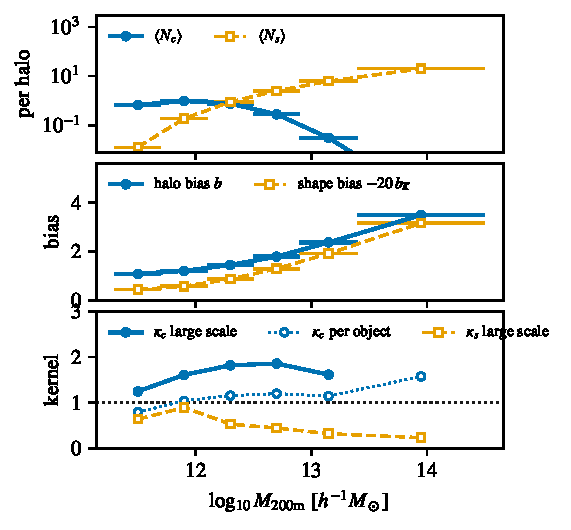
\includegraphics[width=0.55\linewidth]{plots/ingredients/ingredients.pdf}
\caption{The galaxy layer and the large-scale gravity layer at $z=1$ per
host-mass bin (horizontal bars: bin widths, clipped for drawing). Top: mean
centrals and satellites per halo. Middle: halo bias $b$ and halo-shape bias
$\bK$ (scaled by $-20$). Bottom: alignment kernels; solid, large-scale
(on the mean-HOD fields); dotted, per-object central regression. The
central kernel of the most massive bin is left out (fewer than 0.01
sample centrals per halo).}
\label{fig:ingredients}
\end{figure}

% =====================================================================
\section{The gravity layer: halo shapes are strongly nonlinear}
\label{sec:gravity}
% =====================================================================

The first halo models of IA put the 2-halo shape term on $\Plin$, and the
next ones multiplied it by the nonlinear halo bias of Dark Emulator,
$1+\bNL$. Both assume that halo shapes respond to nonlinear gravity like
halo densities. Figure~\ref{fig:shape} shows that they do not. The
galaxy-weighted shape-position spectrum rises above its linear-bias value
about as fast as matter does, while the halo density saturates near
$k\sim1\hMpc$ (halo exclusion) and so does $\bNL$. A shape is a quadrupole
of the mass distribution inside a halo, set by the tidal field and by
anisotropic accretion on the scale of the halo; it keeps gaining power
where densities stop. This is why the HMc and $\bNL$ models of the
previous note could not reach $k\sim1$ without a free $\alpha$ that made up
the missing power.

\begin{figure}[t]
\centering
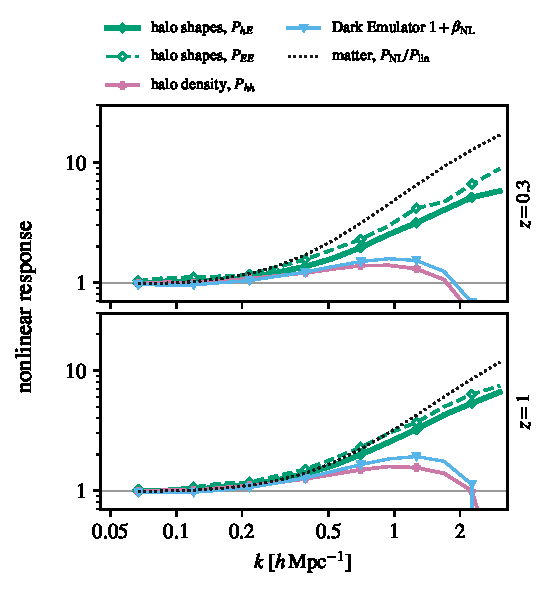
\includegraphics[width=0.55\linewidth]{plots/shape_response/shape_response.pdf}
\caption{Nonlinear response of the gravity layer, galaxy weighted (each
curve a 2-halo sum over host-mass bins divided by the same sum with linear
biases on $\Plin$), at $z=0.3$ and 1. Halo-shape GI and II against halo
density, the Dark Emulator $1+\bNL$ on the same weights and the matter
$\PNL/\Plin$ of FLAMINGO.}
\label{fig:shape}
\end{figure}

% =====================================================================
\section{Three corrections of the galaxy layer}
\label{sec:two}
% =====================================================================

\paragraph{Weight halos by the mean HOD.} A first version weighted every
halo of a mass bin equally. Inside a bin galaxies sit in the more
massive, more biased halos, and the model galaxy density missed
$\refresh{\ggBinnedMiss}$ percent of the large-scale $P_{gg}$ at $z=1$
(Fig.~\ref{fig:weighting}, top). Weighting each halo by $\Nc(M)$ and
$\Ns(M)$ at its own mass, the discrete form of the halo model's mass
integral, recovers most of it; the remaining $\refresh{\ggMeanMiss}$
percent disappears only with each halo's actual occupation, so it is
assembly bias (galaxy occupation correlated with environment at fixed
mass). The kernels are calibrated on GI through this density, so a
wrong galaxy bias would move into $\kappa$ and then, squared, into II.

\paragraph{Galaxies inherit the two parts of the halo shape differently.}
With kernels calibrated on GI, $\kappa^2$ times the full halo-shape II
over-predicts the galaxy II by $\refresh{\iiFullExcess}$ percent at
$k=0.1$ to $0.5\hMpc$ and $z\le1$ (Fig.~\ref{fig:weighting}, bottom),
while the deterministic II alone matches it within
$\refresh{\iiDetDev}$ percent: at low redshift galaxies inherit the tidal
response of their halo and little of its residual shape. The first version
of this note therefore used the deterministic II alone. At $z=2$ that
fails: the galaxy 2-halo II exceeds the deterministic II by
$\refresh{\iiDetExcessTwo}$ percent and even $\kappa^2$ times the full
halo-shape II by $\refresh{\iiFullExcessTwo}$ percent at $k=0.1$ to
$0.55\hMpc$ (Fig.~\ref{fig:residual}, bottom), and the galaxies show a
2-halo $B$ mode that the deterministic term cannot have.

Both regimes are one statement once the residual has its own kernel,
Eq.~\eqref{eq:kernel}. The object-level regression measures it with no
reference to the spectra, and its ratio to the large-scale kernel rises
smoothly with redshift (Fig.~\ref{fig:residual}, top): for centrals it is
$\refresh{\krcZero}$ at $z=0$, $\refresh{\krcOne}$ at $z=1$,
$\refresh{\krcTwo}$ at $z=2$ and $\refresh{\krcFour}$ at $z=4$
(satellites $\refresh{\krsOne}$ at $z=1$). The residual term of
Eq.~\eqref{eq:ii} enters with $(\kappa^r/\kappa^d)^2$, about 0.3 at low
redshift, where it is a small addition, and 0.7 at $z\ge2$, where
galaxies follow nearly all of their halo's shape. It removes about half of
the $z=2$ excess, leaving $\refresh{\iiResExcessTwo}$ percent, which the
kernel gradient takes up (Section~\ref{sec:checks}). One reading, not
tested here: at high redshift a galaxy and its halo's present shape grew
from the same recent anisotropic inflow, while at low redshift the
galaxy's shape was set early and has decoupled from later changes of the
outer halo.

\begin{figure}[t]
\centering
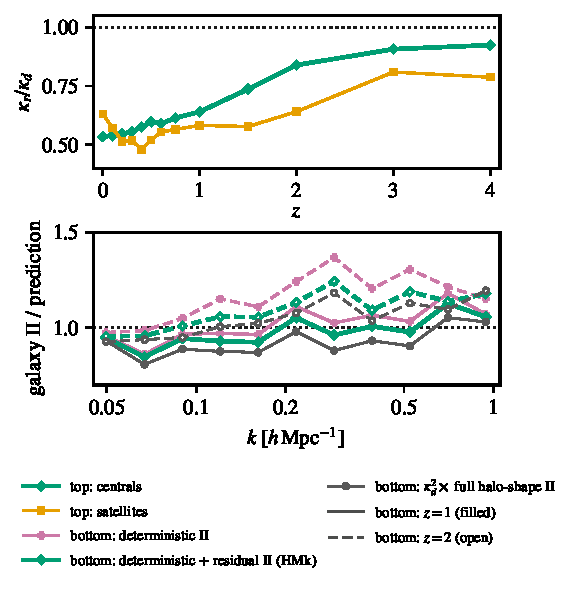
\includegraphics[width=0.55\linewidth]{plots/residual/residual.pdf}
\caption{Top: object-level over large-scale kernel, $\kappa^r/\kappa^d$,
weighted by the number of centrals or satellites per host-mass bin.
Bottom: the measured 2-halo galaxy II (measured $P_{EE}$ minus the measured
1-halo term) over three 2-halo predictions: the deterministic II, the
deterministic plus residual II of Eq.~\eqref{eq:ii} (HMk without the
kernel gradient) and $\kappa_d^2$ times the full halo-shape II. Solid,
filled: $z=1$; dashed, open: $z=2$.}
\label{fig:residual}
\end{figure}

\paragraph{Let the kernel saturate.} The first version fitted
$\kappa\to\kappa(1+\alpha k^2)$. At $z\le1.5$ that worked, but at $z\ge2$
$\alpha$ fell by at least $\refresh{\alphaShiftHigh}\,h^{-2}{\rm Mpc}^2$
(up to $\refresh{\alphaShiftHighSig}\,\sigma$) between $\kmax=0.52$ and
1.26, and still by $\refresh{\alphaShiftHighSigK}\,\sigma$ with the residual
term in place: the measured GI excess grows more slowly than $k^2$ above
$k\sim1/R_L$. The saturating form of Eq.~\eqref{eq:grad}, with $R_L$ taken
from the host masses, follows it with the same single amplitude
(Section~\ref{sec:checks}).

\begin{figure}[t]
\centering
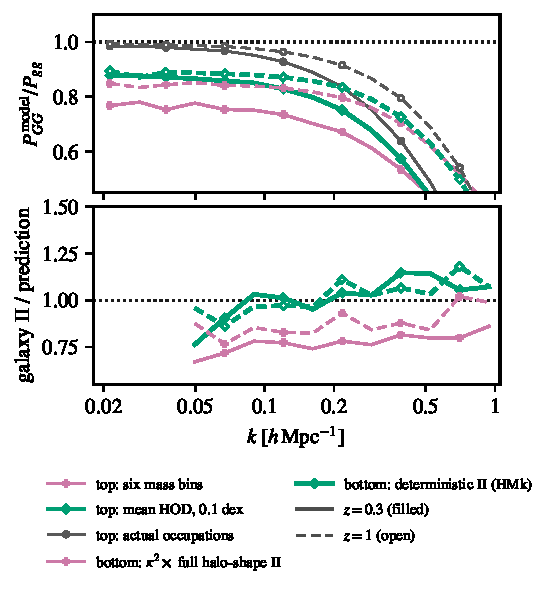
\includegraphics[width=0.55\linewidth]{plots/weighting/weighting.pdf}
\caption{Top: model galaxy density power over the measured $P_{gg}$ for
three halo weightings. Bottom: the measured 2-halo galaxy II (measured
$P_{EE}$ minus the measured 1-halo term) over $\kappa^2$ times the full
halo-shape II and over the deterministic halo-shape II, Eq.~\eqref{eq:ii}.
Solid: $z=0.3$; dashed, open markers: $z=1$.}
\label{fig:weighting}
\end{figure}

% =====================================================================
\section{Goodness of fit on FLAMINGO}
% =====================================================================

Figure~\ref{fig:spectra} shows the spectra at $z=1$ and 2. Without a
fitted parameter (dashed) the model follows $P_{hE}$ to about
$0.3\hMpc$ and then falls short, by 5 to 10 percent at $z=1$ and 10 to 20
percent at $z=2$; $P_{EE}$ and $P_{BB}$ follow within a few $\sigma$ to
$k\sim1$, with the close-pair (1-halo) term carrying $P_{BB}$ and most of
$P_{EE}$ above $0.5\hMpc$. The kernel gradient closes the $P_{hE}$ gap
and the remaining $P_{EE}$ deficit at $z=2$ (solid).

\begin{figure}[t]
\centering
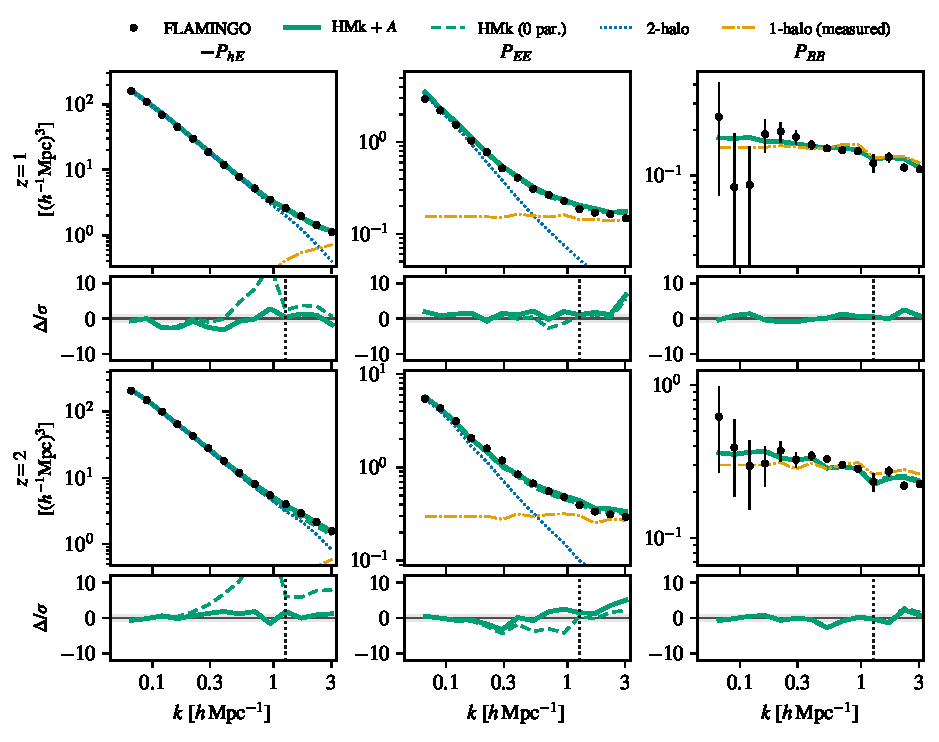
\includegraphics[width=\linewidth]{plots/spectra/spectra.pdf}
\caption{FLAMINGO spectra (points) at $z=1$ and 2 with HMk without a
fitted parameter (dashed), HMk with the saturating kernel gradient fitted
to $k\le\Kfit\hMpc$ (solid, dotted vertical line), and the 2-halo and
1-halo parts of the former. Residual rows: (model $-$ data)$/\sigma$, the
grey band $\pm1$.}
\label{fig:spectra}
\end{figure}

Figure~\ref{fig:gof} puts all variants side by side. The goodness-of-fit
cut (median over $z$) is $\refresh{\cutLinMed}\hMpc$ for the linear gravity
layer, $\refresh{\cutEmuMed}$ for the density $\bNL$ and
$\refresh{\cutTabMed}$ for the binned version with full II. HMk without
a fitted parameter has summed $\chi^2/\nu=\refresh{\gofWA}$ at
$\kmax=0.52$ and $\refresh{\gofWC}$ at 0.94; with the kernel gradient
these are $\refresh{\gofWgA}$ and $\refresh{\gofWgC}$ (the first version:
$\refresh{\gofVoneA}$ and $\refresh{\gofVoneC}$), against
$\refresh{\gofTattA}$ and $\refresh{\gofTattC}$ for TATT with four fitted
parameters. The cut of HMk without a fitted parameter is
$\refresh{\cutWLo}$ to $\refresh{\cutWHi}\hMpc$ (median $\refresh{\cutWMed}$);
with $A$ it is
$\refresh{\cutWgLo}$ to $\refresh{\cutWgHi}\hMpc$ (median
$\refresh{\cutWgMed}$), of TATT $\refresh{\cutTattLo}$ to
$\refresh{\cutTattHi}$ (median $\refresh{\cutTattMed}$). The gain is at
high redshift: at $z=2$, 3 and 4 the cut is $\refresh{\cutWgZTwo}$,
$\refresh{\cutWgZThree}$ and $\refresh{\cutWgZFour}\hMpc$, against
$\refresh{\cutVoneZTwo}$, $\refresh{\cutVoneZThree}$ and none for the
first version, and $\chi^2/\nu$ at $\kmax=0.94$ falls from
$\refresh{\gofVoneZTwo}$, $\refresh{\gofVoneZThree}$, $\refresh{\gofVoneZFour}$
to $\refresh{\gofWgZTwo}$, $\refresh{\gofWgZThree}$, $\refresh{\gofWgZFour}$.
At $z\le1.5$ the two versions differ by at most one step of the $\kmax$
grid either way; the lowest cut is at $z=0.6$, where the data sit below
every model at $k<0.2$ (Fig.~\ref{fig:gof}, right).

\begin{figure}[t]
\centering
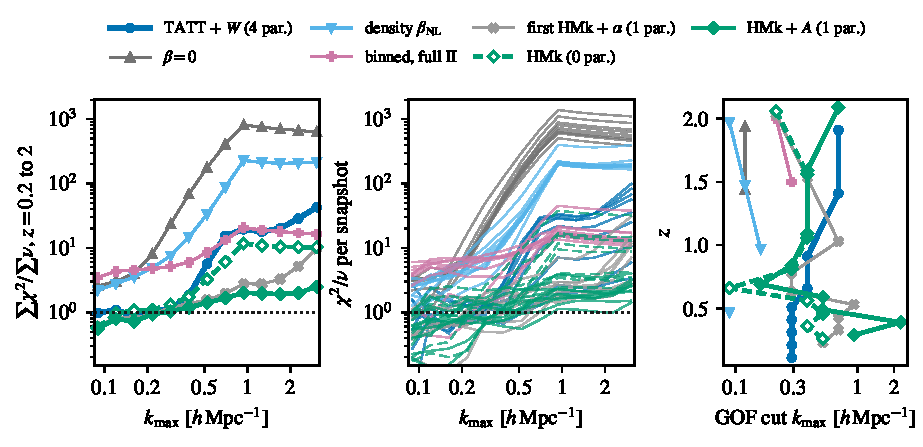
\includegraphics[width=\linewidth]{plots/gof/gof.pdf}
\caption{Goodness of fit against $\kmax$. Left: $\chi^2/\nu$ summed over the
\NsnapCore\ core snapshots. Middle: per snapshot. Right: goodness-of-fit
cut per redshift (points offset in $z$ for legibility). HMk variants fit no
parameter except the kernel gradient ($A$, or $\alpha$ for the first
version: deterministic II and $(1+\alpha k^2)$); TATT (from the previous
note) fits $A_1$, $A_2$, $b_{\rm TA}$ and a white term.}
\label{fig:gof}
\end{figure}

% =====================================================================
\section{Physical checks}
\label{sec:checks}
% =====================================================================

\paragraph{The kernel gradient.} $A$ is the fractional change of the
kernel well inside the host's Lagrangian patch, so its natural size is
well below 1. At $z=0.2$ to 1.5 it is $\refresh{\ALo}$ to $\refresh{\AHi}$
for $\kmax=0.94$ and 1.26, and at $z\ge2$ about $\refresh{\AHighFit}$
(Fig.~\ref{fig:checks}, top). It is positive at every redshift: galaxies
follow small-scale tides somewhat more closely than their halos' dark
matter does. From $\kmax=0.52$ to 1.26 it moves by at most
$\refresh{\AShiftMid}$ at $z\le1.5$ and $\refresh{\AShiftHigh}$ at
$z\ge2$, at most $\refresh{\AShiftSig}\,\sigma$ of its error at
$\kmax=0.52$, where the first version's $\alpha$ moved by up to
$\refresh{\alphaShiftHighSig}\,\sigma$: the check passes, loosely (a few
$\sigma$ in a single box with sub-percent errors at $k\sim1$). Above the fit
range the gradient is bounded by construction, $1+A$, so the model cannot
run away at $k>\Kfit$. The rise of $A$ with redshift tracks the rise of
$\kappa^r/\kappa^d$ (Fig.~\ref{fig:residual}): both say that galaxies at
high redshift follow their halo's shape, and the small-scale tides, more
closely.

\paragraph{The residual term.} Its kernels come from a regression, not a
fit, and the deterministic II computed from the split fields equals the
first version's to $10^{-4}$ (Appendix~\ref{app:checks}). Its size
follows $(\kappa^r/\kappa^d)^2$: at $k\approx0.3\hMpc$ it adds 3 to 10
percent to the deterministic II at $z\le2$ and 25 to 50 percent at $z=3$
and 4. It is not positive everywhere. Below $k=0.1\hMpc$ it is the
difference of two noisy spectra on a few hundred modes and takes its
$k\to0$ limit there, a constant (the mean over $k=0.1$ to 0.2), as the
1-halo term does. At $k=0.1$ to $1.3\hMpc$ it dips below zero by at most
$\refresh{\negIIMax}$ percent of the model $P_{EE}$, and the 2-halo $B$
mode by at most $\refresh{\negBBMax}$ percent of the model $P_{BB}$, near
$k\sim1$: the 2-halo shape correlation of distinct halos can turn negative
on the scale of their exclusion, and the noise subtraction leaves a
percent-level scatter.

\paragraph{The kernels.} $\kc$ and $\ks$ vary smoothly with $z$ and mass
(Fig.~\ref{fig:checks}), except in the bins with the fewest galaxies
(satellites of the lowest-mass hosts, at under one per hundred halos), which
are noisy and carry little weight. $\kc>1$ is allowed
(Eq.~\ref{eq:kernel}). The
template amplitudes $\Aeff$ rise from $\refresh{\AeffLo}$ at $z=0$ to
$\refresh{\AeffHi}$ at $z=4$, those of the FLAMINGO truth.

\begin{figure}[t]
\centering
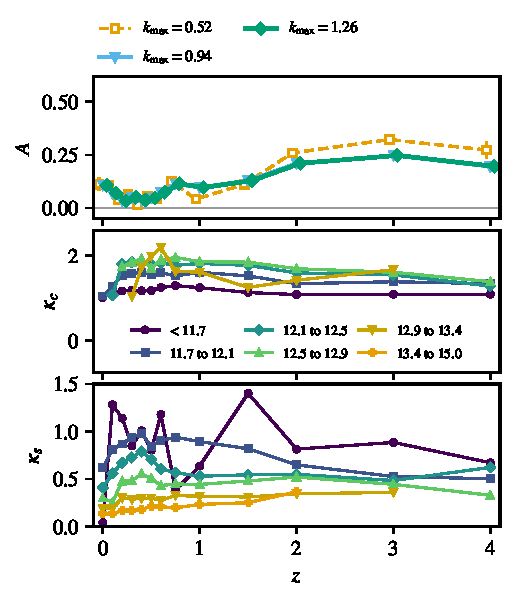
\includegraphics[width=0.55\linewidth]{plots/checks/checks.pdf}
\caption{Top: the saturated kernel gradient $A$ of Eq.~\eqref{eq:grad}
per snapshot for three $\kmax$, with $1\sigma$ errors from the $\chi^2$
curvature. Middle and bottom: large-scale central and satellite kernels
per host-mass bin [$\log_{10}M_{\rm 200m}$] against $z$.}
\label{fig:checks}
\end{figure}

% =====================================================================
\section{Figure of bias for Roman}
% =====================================================================

The model enters Roman as native NLA($A_1$, $\eta_1$) plus a template that
turns the NLA shape into the HMk shape at each snapshot, exact in the
amplitude and held at the fiducial cosmology:
\begin{equation}
\xi = \xi_{\rm NLA}(A_1,\eta_1) + \sum_s\left[A_s\,U^{\rm GI}_s + A_s^2\,U^{\rm II}_s\right],
\qquad A_s = A_1\left(\frac{1+z_s}{1.62}\right)^{\eta_1},
\end{equation}
where $U_s$ is the data-vector response to (HMk shape $-$ NLA shape) per
unit amplitude, so that at $A_s=A_{{\rm eff},s}$ the data vector is the HMk
prediction. The template uses the model where it was tested,
$0.2\le k\le\Kfit\hMpc$, and holds its ratio to the truth constant outside:
below $k=0.2$ every halo model is NLA, and the single box's cosmic variance
(the data lie 4 to 19 percent above the smooth truth at $k<0.15$) would
otherwise set the template's amplitude. A first construction that took
the amplitude from $k=0.03$ to 0.10 and the model to $k=3$ gave
$\refresh{\fobVoneCsWgTwo}$ at $K_0=0.2$ and $\refresh{\fobVoneCsWgEight}$ at
0.8 (Appendix~\ref{app:checks}). The template takes the final model with
$A$ fitted to $k\le\Kfit\hMpc$ at each snapshot. The matched control uses
the truth's own shape in place of HMk: its bias measures what the
power-law amplitude alone costs. Diagnostics use a model at $z\le1.5$ and
the truth's own shape above, to see where the bias enters.

Figure~\ref{fig:fob} gives the result. In cosmic shear the control stays
at $\refresh{\fobCsCtrlLo}$ to $\refresh{\fobCsCtrlHi}$ for every $K_0$ to
0.8. HMk stays below 0.3 to $K_0=\refresh{\KzeroCsWg}$ and reaches
$\refresh{\fobCsWgEight}$ at 0.8, against $\refresh{\fobCsVoneEight}$ for
the first version, $\refresh{\fobCsNlaEight}$ for NLA and
$\refresh{\fobCsTattEight}$ for TATT. Without the kernel gradient (dashed)
it gives $\refresh{\fobCsWEight}$: in Roman the gradient matters little.
The $z\ge2$ problem of the first version is gone: HMk with the truth's
shape above $z=1.5$ gives $\refresh{\fobCsKzEight}$ at 0.8, the same as HMk
everywhere. What is left comes from $z\le1.5$, and the diagnostics locate
it in the residual term. At $z\le1.5$ (truth above), the saturating
gradient on the deterministic II gives $\refresh{\fobCsDiagSatEight}$, as
the first version did ($\refresh{\fobCsVoneKzEight}$), while the residual
term with the $k^2$ gradient gives $\refresh{\fobCsDiagResEight}$. The
residual term thus trades a cost of about 0.05 at $z\le1.5$ for the gain
at $z\ge2$; on FLAMINGO the two versions fit $z\le1.5$ equally well, so
the spectra do not decide this trade.

In 3x2pt the control itself crosses 0.3 at $K_0=\refresh{\KzeroTxCtrl}$,
so the amplitude's redshift evolution, not the shape, limits the 3x2pt
cut. HMk gives $\refresh{\fobTxWgLo}$ to $\refresh{\fobTxWgHi}$, below the
control at every $K_0$: its shape error partly cancels the bias of the
power-law amplitude. That is a coincidence of signs, not a better shape.

\begin{figure}[t]
\centering
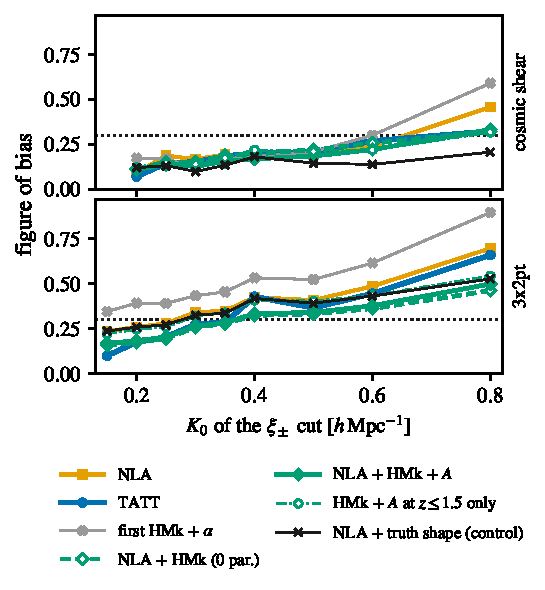
\includegraphics[width=0.55\linewidth]{plots/fob_k0scan/fob_k0scan.pdf}
\caption{Roman figure of bias against the $\xi_\pm$ cut $K_0$ (CP truth,
CMB prior, Fisher shift of $\Omega_m$, $S_8$). Top: cosmic shear; bottom:
3x2pt ($\gamma_t$ at 0.5, $w$ at 0.2). NLA + HMk: the final template
without (dashed) and with the kernel gradient $A$; dash-dotted: HMk at
$z\le1.5$ and the truth's own shape above; grey: the first version of
this note (deterministic II, $k^2$ gradient); control: the template of the
truth's own shape at every $z$. Dotted: 0.3.}
\label{fig:fob}
\end{figure}

\clearpage
\appendix

% =====================================================================
\section{Numerical checks}
\label{app:checks}
% =====================================================================

\paragraph{Estimator.} The halo-kernel estimator reproduces the FLAMINGO
pipeline's own spectra at $z=1$ to 0.1 percent ($P_{hh}$, $P_{hE}$) and
0.6 percent ($P_{BB}$) in fold 1. On the fit grid the catalogue
measurement of the galaxies agrees with the fitted data to
$\refresh{\reproLow}\,\sigma$ below $k=0.52$; at $k=0.7$ to 0.94, the top of
fold 1 on the \NGmesh\ mesh, it differs by up to $\refresh{\reproHigh}\,\sigma$
(1 to 5 percent), which is aliasing of the coarser mesh. The model is
compared with the data after adding this offset.

\paragraph{Split fields.} The deterministic II computed from the fields of
the split, $P_{H,E^d}^2/P_{HH}$, equals that of the first version (built
bin by bin) to $10^{-4}$ at every $k$ and snapshot, so the two codes agree
on the shared term. The self-pair noise of $P_{E^rE^r}$ and $P_{B^rB^r}$
is the same spectrum measured with every halo shape rotated by an
independent random angle, which keeps the weights and the window and
removes every correlation between halos.

\paragraph{Mean HOD.} The weights preserve the number of galaxies in every
\dlgM-dex bin exactly; galaxies in hosts below $10^{\Mcomp}\Msun$ (3
percent) keep their halos' actual counts.

\paragraph{Templates.} The template of the truth's own shape reproduces
the CP data vector at the truth's amplitudes to $\chi^2<10^{-13}$. A first
version held the model ratio, not its ratio to the truth, constant
outside $k=0.05$ to 3.1, which already cost $\chi^2=1.7$ at $K_0=0.3$ for
the truth's own shape; the model's ratio to the truth is now held instead.
Taking the HMk amplitude from its own low-$k$ values, where it inherits the
box's cosmic variance, and the model to $k=3$ (where $\alpha k^2$ and the
deterministic II both overshoot) gave a cosmic-shear figure of bias of
$\refresh{\fobVoneCsWgTwo}$ to $\refresh{\fobVoneCsWgEight}$; the adopted
construction uses the model on $0.2\le k\le\Kfit\hMpc$.

% =====================================================================
\section{Where the code and results are}
% =====================================================================

\begin{center}
\footnotesize
\setlength{\tabcolsep}{3pt}
\begin{tabular}{ll}
\toprule
result & script (output) \\
\midrule
halo catalogue & \texttt{flamingo/extraction/soap\_halos.py} (\texttt{SOAP\_halos/halos\_<sn>.hdf5}) \\
binned kernels, 1-halo & \texttt{analysis/halo\_kernel/hk\_measure.py} (\texttt{kernels\_<sn>.npz}) \\
mean-HOD halo fields & \texttt{analysis/halo\_kernel/hk\_weighted.py} (\texttt{weighted\_<sn>.npz}) \\
split fields & \texttt{analysis/halo\_kernel/hk\_stoch.py} (\texttt{stoch\_<sn>.npz}) \\
model (final: \texttt{ws-ls-sat}), GOF & \texttt{analysis/halo\_kernel/hk\_model.py} (\texttt{model/hk\_model.json}) \\
Roman templates & \texttt{analysis/halo\_kernel/hk\_templates.py} (\texttt{hm\_templates\_*\_CP.npz}) \\
figure of bias & \texttt{analysis/cut\_validation/fisher\_minimize.py} (models NLAs, NLAs0, NLAsz, \\
 & NLAk, NLAt, NLAd1, NLAd2; job files \texttt{jobs\_hms*.txt}, \texttt{jobs\_hmd.txt}) \\
\bottomrule
\end{tabular}
\end{center}

% =====================================================================
\section{Open issues}
% =====================================================================

\paragraph{Gravity layer over cosmology.} The halo spectra are tabulated
from FLAMINGO at one cosmology. A Roman analysis that varies cosmology
needs them as a function of cosmology, i.e.\ a shape analogue of Dark
Emulator trained on dark-matter-only halos; the shape response of
Fig.~\ref{fig:shape} is the target.

\paragraph{1-halo term.} The 1-halo term is measured, not built from the
kernels, the radial alignment and the profile. An analytic 1-halo term
from Eq.~\eqref{eq:kernel} is the next step for portability.

\paragraph{Assembly bias.} The mean-HOD weighting leaves
$\refresh{\ggMeanMiss}$ percent of $P_{gg}$ at $z=1$; it enters through the
kernel calibration.

\paragraph{Residual kernel.} $\kappa^r$ is the object-level regression,
attenuated by halo-shape measurement noise, so it is a lower limit of how
strongly galaxies inherit the correlated residual; a residual inherited
partly through the tides (with $\kappa^d$) would sit between the
deterministic + residual II and the full II of Fig.~\ref{fig:residual}.
At $z\le1.5$ the residual term costs about 0.05 in the Roman figure of
bias at $K_0=0.8$ while the spectra do not prefer either version there.

\paragraph{Rising kernel gradient.} $A$ doubles from $z\le1.5$ to $z\ge2$,
together with $\kappa^r/\kappa^d$; the saturating form follows the data
but is not derived from galaxy formation. At $z=2$ the 2-halo galaxy II is
still $\refresh{\iiResExcessTwo}$ percent above the deterministic +
residual II before the gradient acts.

\paragraph{Amplitude evolution.} The matched control shows that the
power-law $A(z)$ limits 3x2pt for any shape. A freer $A(z)$ combined with
the HMk template has not been run.

\paragraph{Second suite.} The galaxy layer has not been recalibrated on
TNG300 to test whether one gravity layer serves both suites.

\end{document}
